\chapter{أدلة التطور}\label{ch:g9:evidence-of-evolution}

وقف هذا الكتاب مرتين على حافة دعوى كبيرة: فروع \omterm{def:g6:classification-kinship:tree}{شجرة
القرابة} كلها تلتقي
(\cref{rem:g6:classification-kinship:implies})، وكل \omterm{def:g6:exploring-our-environment:components}{كائن
حي} يقرأ شفرة واحدة
(\cref{rem:g9:genes-and-dna:universal}). وللدعوى التي
تشيران إليها اسم --- هو \emph{التطور}: \omterm{def:g5:biodiversity:species}{الأنواع} تتغير عبر
الأجيال، وكلها منحدرة من أسلاف مشتركين. وقبل أن يسأل
الفصل التالي \emph{كيف}، يفعل هذا الفصل ما طالب به
\cref{exo:g6:classification-kinship:12}: يبسط الأدلة.

\section{شهادة الصخور}

\begin{definition}[الأحافير]\label{def:g9:evidence-of-evolution:fossils}
\emph{الأحفورة}\index{أحفورة} أثر محفوظ من حياة ماضية ---
\omterm{def:g1:animals-around-us:covering}{صدفة}، أو \omterm{def:g3:bones-and-muscles:skeleton}{عظم}، أو بصمة \omterm{def:g1:plants-around-us:parts}{ورقة}، أو أثر قدم --- مختوم في صخر
رسوبي. وطبقات الصخر تتراكم بترتيب الزمن، أقدمها أسفلها؛
فقراءتها صعودًا قراءة للتاريخ. والأحافير هي نصف البقايا
من جرد
\cref{def:g6:exploring-our-environment:components}،
محفوظًا ملايين السنين.
\end{definition}

\begin{proposition}[ما يبينه السجل المتطبق]\label{prop:g9:evidence-of-evolution:record}
مقروءًا بترتيبه، يشهد السجل ثلاث مرات:
\begin{enumerate}
  \item \emph{\omterm{def:g1:animals-around-us:animal}{الحيوانات} تتغير}: فلكل عمر من أعمار
        الطبقات شخوصه --- فلا أرانب بين ثلاثيات الفصوص،
        ولا ثلاثيات فصوص في طبقات الأرانب؛ وأكثر \omterm{def:g5:biodiversity:species}{أنواع}
        كل طبقة عميقة \emph{منقرضة} (كلمة
        \cref{prop:g5:biodiversity:loss}، ووراءها الآن
        الزمن السحيق)؛
  \item \emph{والترتيب متعشش كالشجرة}: \omterm{prop:g3:sorting-living-things:groups}{فالأسماك} تظهر في
        الطبقات العميقة، وأقرباء \omterm{prop:g3:sorting-living-things:groups}{البرمائيات} ذوات \omterm{def:g1:my-body:parts}{الأطراف}
        الأربعة فوقها، وأقرباء \omterm{prop:g4:classifying-animals:classes}{الزواحف} فوق أولئك،
        \omterm{prop:g3:sorting-living-things:groups}{والثدييات} \omterm{prop:g3:sorting-living-things:groups}{والطيور} أعلى بعد --- فعلب \omterm{def:g4:classifying-animals:classification}{التصنيف}
        (\cref{pb:g6:classification-kinship:1}) تتراكم
        في الزمن تمامًا كما تتنبأ \omterm{prop:g6:classification-kinship:kinship}{القرابة}؛
  \item \emph{والوسائط موجودة}: فلوح
        \emph{الأركيوبتيريكس} الشهير --- \omterm{def:g1:animals-around-us:covering}{ريش} وجناحان على
        هيكل زاحف مسنن طويل الذنب العظمي --- يقف حيث
        يفترق فرعا \omterm{prop:g3:sorting-living-things:groups}{الطيور} \omterm{prop:g4:classifying-animals:classes}{والزواحف}؛ وحيتان أحفورية \omterm{def:g1:my-body:parts}{بأرجل}
        خلفية عاملة تقف حيث طالب بها انحدار
        \cref{ex:g6:classification-kinship:whale} من
        ثدييات اليابسة.
\end{enumerate}
\end{proposition}
\admitted

\begin{example}[سلسلة الحيتان]\label{ex:g9:evidence-of-evolution:whales}
ملف الحوت، وقد ملأته الصخور: \omterm{def:g9:evidence-of-evolution:fossils}{أحافير} متعاقبة، بترتيب
الزمن، تمتد من ثدي شاطئي رباعي \omterm{def:g1:my-body:parts}{الأرجل} بحجم الذئب،
مرورًا بصور تتقلص \omterm{def:g1:my-body:parts}{أرجلها} وتقوى أذنابها، إلى سابحات كاملة
بلا \omterm{def:g1:my-body:parts}{أرجل} --- بينما لا يزال حوت اليوم يبني \omterm{def:g3:bones-and-muscles:skeleton}{عظام} ورك \omterm{def:g1:my-body:parts}{ورجل}
صغيرة مخفية (وقد لاحظ
\cref{ex:g6:classification-kinship:placing} الأعضاء
الأثرية) ولا يزال يرضع ويتنفس الهواء وينبت شعرًا
جنينيًا. تنبؤ، \omterm{def:g9:evidence-of-evolution:fossils}{وأحافير}، وأعضاء أثرية: ثلاثة مفاتيح، وقفل
واحد.
\end{example}

\begin{omfigure}
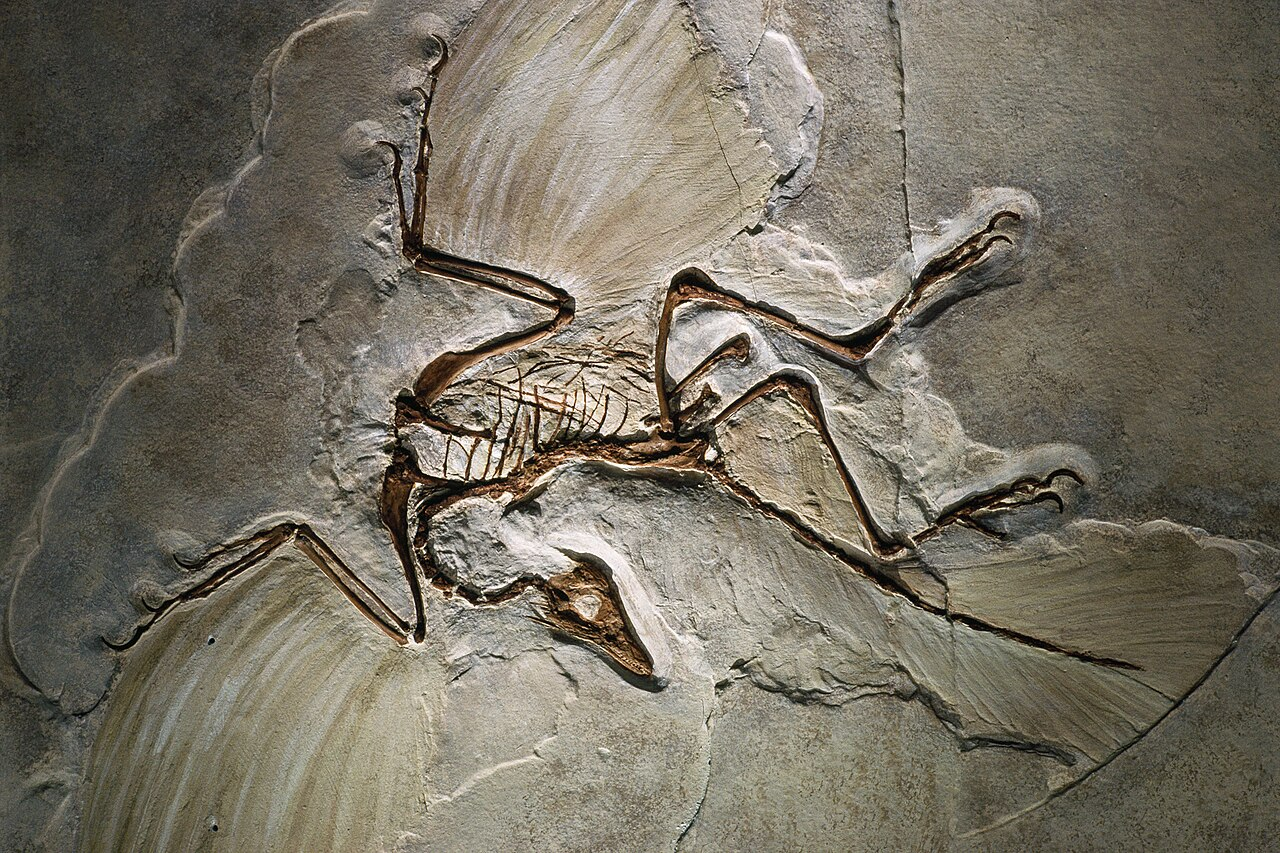
\includegraphics[width=0.62\linewidth]{images/book1/archaeopteryx.jpg}

{\small \omterm{def:g9:evidence-of-evolution:fossils}{أحفورة} \emph{الأركيوبتيريكس}: جناحان مريشان على
هيكل زاحف مسنن طويل الذنب --- وسيط يقف حيث تفترق فروع
الشجرة.}
\end{omfigure}

\section{شهادة الأجسام الحية}

\begin{proposition}[التشريح يتذكر]\label{prop:g9:evidence-of-evolution:anatomy}
الأجسام الحية تحمل تاريخها:
\begin{itemize}
  \item \emph{المخطط المشترك}: فجناح الخفاش، وزعنفة
        الحوت، \omterm{def:g1:my-body:parts}{ورجل} الحصان، وذراعك ترتيب عظمي واحد (فرع
        \omterm{def:g1:my-body:parts}{الأطراف} الأربعة في
        \cref{pb:g6:classification-kinship:1}) مُطّ
        وقُصّر وأعيدت وظيفته --- \omterm{def:g9:heredity-and-traits:heredity}{فالوراثة} تفسر ما لا
        تكرره هندسة جديدة أبدًا؛
  \item \emph{والأعضاء الأثرية}: وركا الحوت، وجناحا
        الخنفساء غير الطائرة الملحومان، وعصعصك أنت، وحال
        الزائدة الدودية الضامرة --- أجزاء أبقيت لأن
        الانحدار يبني على القائم، لا من الصفر؛
  \item \emph{\omterm{def:g5:human-reproduction:pregnancy}{والمضغ} تتفق}: \omterm{def:g5:human-reproduction:pregnancy}{فمضغ} \omterm{def:g4:classifying-animals:vertebrate}{الفقاريات} من سمكة وفرخ
        وإنسان تجري متشابهة تشابهًا لافتًا خلال أسابيعها
        الأولى (وضع المخطط في
        \cref{prop:g8:from-egg-to-birth:timetable}) ---
        تعليمات بناء مشتركة، تفترق متأخرة.
\end{itemize}
\end{proposition}
\admitted

\begin{proposition}[الجزيئات تصوّت]\label{prop:g9:evidence-of-evolution:molecules}
وأحدث الشهود شفرة
\cref{rem:g9:genes-and-dna:universal}. قارن تهجئة مورّثة
واحدة محفوظة جيدًا عبر \omterm{def:g5:biodiversity:species}{الأنواع}: فالإنسان والشمبانزي
يختلفان في أحرف قليلة، والإنسان والفأر في أكثر، والإنسان
والسمكة في أكثر بعد، والإنسان \omterm{ex:g6:producing-our-food:bread}{والخميرة} في الأكثر ---
والمسافات، محصاة مورّثة بعد مورّثة، تعيد رسم
\emph{الشجرة نفسها} التي رسمها التشريحيون من \omterm{def:g3:bones-and-muscles:skeleton}{العظام}
ورسمها علماء \omterm{def:g9:evidence-of-evolution:fossils}{الأحافير} من الطبقات. ثلاثة شهود مستقلين،
وشجرة عائلة واحدة: وذلك الاتفاق هو سبب كف البيولوجيين
عن الجدال في \emph{هل}، والتفاتهم إلى \emph{كيف}.
\end{proposition}
\admitted

\begin{example}[أن تراه يتحرك]\label{ex:g9:evidence-of-evolution:live}
بل التغير يرى حيث تدور الأجيال سريعًا. فالصورة الداكنة
من عثة الفلفل انتشرت في \omterm{prop:g5:people-and-nature:managed}{الغابات} الصناعية الملطخة
بالسخام، وانحسرت حين صفا الهواء؛ \omterm{prop:g3:sorting-living-things:groups}{والحشرات} المنيعة على
المبيدات \omterm{def:g6:producing-our-food:fermentation}{والميكروبات} المتحدية للمضادات الحيوية
(\cref{ch:g9:microbes-and-infection} سيلقى الحالة
الطبية) تنشأ في غضون سنوات؛ وتوزيعات حجم مناقير عصافير
الجزر تنزاح مع الجفاف والوفرة، مقيسة حية بدراسات التحليق
والفرجار. حركات صغيرة، وأزمنة قصيرة --- الآلية ملتقطة
وهي تعمل، مهما كان مداها في الأمد الطويل.
\end{example}

\begin{method}[وزن الدليل التاريخي]\label{met:g9:evidence-of-evolution:weigh}
التطور تاريخ، والدعاوى التاريخية تختبر كما تختبر القضية
القديمة في \cref{pb:g9:unique-individuals:1} --- بتقارب
شهود مستقلين:
\begin{enumerate}
  \item اسأل بم \emph{تتنبأ} الدعوى: أي وسائط، وأي أعضاء
        أثرية، وأي مسافات جزيئية؛
  \item وتحقق من كل شاهد على حدة: الصخور، والأجسام،
        والجزيئات، والمراقبات الحية؛
  \item وزن استقلالها: فالشهود الذين لا يمكن أن يكونوا
        قد تواطؤوا، إذا اتفقوا، ضاعفوا المصداقية؛
  \item وأبق الحكم مفتوحًا للاكتشاف التالي --- ولاحظ حين
        تظل الاكتشافات تحل حيث قالت الدعوى أن نحفر
        (\omterm{def:g1:my-body:parts}{فأرجل} الحيتان طلبت، فوجدت).
\end{enumerate}
\end{method}

\section{تمارين}

\begin{exercise}[$\star$]\label{exo:g9:evidence-of-evolution:1}
ما \omterm{def:g9:evidence-of-evolution:fossils}{الأحفورة}، ولماذا تقرأ طبقات الصخر خطًا زمنيًا؟
\end{exercise}

\begin{exercise}[$\star$]\label{exo:g9:evidence-of-evolution:2}
اذكر شهادات السجل المتطبق الثلاث.
\end{exercise}

\begin{exercise}[$\star$]\label{exo:g9:evidence-of-evolution:3}
أي خليط من السمات يجعل \emph{الأركيوبتيريكس} وسيطًا؟
\end{exercise}

\begin{exercise}[$\star$]\label{exo:g9:evidence-of-evolution:4}
أعط ثلاثة أعضاء أثرية وبم يشهد كل واحد منها.
\end{exercise}

\begin{exercise}[$\star$]\label{exo:g9:evidence-of-evolution:5}
كيف تعيد المقارنات الجزيئية رسم الشجرة؟
\end{exercise}

\begin{exercise}[$\star$]\label{exo:g9:evidence-of-evolution:6}
سمّ مراقبتين حيتين للتغير من
\cref{ex:g9:evidence-of-evolution:live}.
\end{exercise}

\begin{exercise}[$\star\star$]\label{exo:g9:evidence-of-evolution:7}
لماذا يحتج مخطط \omterm{def:g1:my-body:parts}{الأطراف} المشترك \omterm{def:g9:heredity-and-traits:heredity}{للوراثة} لا لتصميم جيد
أعيد استعماله؟ (ما الذي كانت هندسة جديدة حرة في أن
تفعله؟)
\end{exercise}

\begin{exercise}[$\star\star$]\label{exo:g9:evidence-of-evolution:8}
اجمع ملف الحوت كاملًا: سمات الطائفة، والأعضاء الأثرية،
وسلسلة \omterm{def:g9:evidence-of-evolution:fossils}{الأحافير}، \omterm{prop:g6:classification-kinship:kinship}{والقرابة} الجزيئية --- سطر لكل واحد.
\end{exercise}

\begin{exercise}[$\star\star$]\label{exo:g9:evidence-of-evolution:9}
لماذا يعد \emph{اتفاق} الصخور والأجسام والجزيئات أكثر
قيمة من أي شاهد وحده؟ استعمل خطوة الاستقلال في
\cref{met:g9:evidence-of-evolution:weigh}.
\end{exercise}

\begin{exercise}[$\star\star$]\label{exo:g9:evidence-of-evolution:10}
``لا أرانب بين ثلاثيات الفصوص.'' لماذا كان ذلك الغياب
--- مطردًا في كل حفر أجري قط --- دليلًا قويًا بذاته؟
\end{exercise}

\begin{exercise}[$\star\star$]\label{exo:g9:evidence-of-evolution:11}
شاهد \omterm{def:g5:human-reproduction:pregnancy}{المضغة}: ما الذي يتفق، ومتى يفترق، وآلة أي فصل تقول
لماذا كانت التعليمات الباكرة المشتركة أهم ما يكون؟
\end{exercise}

\begin{exercise}[$\star\star\star$]\label{exo:g9:evidence-of-evolution:12}
اكتب حجة الفصل بوصفها
\cref{met:g9:evidence-of-evolution:weigh} مطبقة كاملة:
الدعوى، والتنبؤات، والشهود الأربعة، والحكم --- والسؤال
الذي يسلّمه الحكم إلى \cref{ch:g9:how-species-change}.
\end{exercise}

\section{مسألة: جناح المتحف الجديد}

\begin{problem}[{مسألة نهاية الأسبوع --- تنسيق قاعة
الأدلة}]\label{pb:g9:evidence-of-evolution:1}
يبني متحف التاريخ الطبيعي جناحًا للتطور، وينسّق الصف
أربع غرف: الصخور، والأجسام، والجزيئات، والمراقبات الحية.

\medskip\noindent\textbf{الجزء الأول --- غرفة غرفة.}
\begin{enumerate}
  \item الصخور: رتّب الجدار --- لوح ثلاثي الفصوص، وأول
        سمكة، وآثار أقدام أقرباء \omterm{prop:g3:sorting-living-things:groups}{البرمائيات}، وهياكل
        زواحف، وقالب \emph{الأركيوبتيريكس}، وفك ثدي مبكر
        --- واكتب تعليق الغرفة في جملة واحدة من
        \cref{prop:g9:evidence-of-evolution:record}.
  \item الأجسام: القطعة المركزية تبسط جناح الخفاش وزعنفة
        الحوت \omterm{def:g1:my-body:parts}{ورجل} الحصان \omterm{def:g1:my-body:parts}{وذراع} الإنسان من حامل هيكل
        واحد. علّق على المخطط المشترك --- وأضف معروضات
        خزانة الأعضاء الأثرية الثلاثة.
  \item الجزيئات: يحصي جدول الجدار فروق أحرف مورّثة
        واحدة: الشمبانزي 1، والفأر 8، والسمكة 24،
        \omterm{ex:g6:producing-our-food:bread}{والخميرة} 41 (أعداد للتوضيح). بم يجب أن تطابق
        شجرة الجدول، كي تعمل الغرفة؟
  \item المراقبات الحية: اختر معروضين من
        \cref{ex:g9:evidence-of-evolution:live} وقل ما
        الذي يبين كل واحد منهما متحركًا.
\end{enumerate}

\medskip\noindent\textbf{الجزء الثاني --- أسئلة
الزوار.}
\begin{enumerate}[resume]
  \item ``لماذا ما تزال القرود موجودة، إن كنا منحدرين من
        أسلاف مشتركين معها؟'' أجب بتفرع الشجرة ---
        أقرباء، لا سلالم
        (\cref{def:g6:classification-kinship:tree}).
  \item ``وأين الحلقات المفقودة؟'' أشر إلى الموجودة ---
        اثنتان من هذا الفصل --- واذكر بين ماذا وماذا
        وقفت كل واحدة.
  \item ``أليس التطور مجرد نظرية؟'' أجب بمنهج الدليل
        التاريخي: ما معنى ``نظرية'' هنا، وما الذي يثبته
        اتفاق الغرف الأربع.
  \item ``أيمكن أن يقلبه حفر الغد؟'' اذكر أي نوع من
        الاكتشافات يفعل ذلك --- أرانب بين ثلاثيات الفصوص
        --- وماذا عنى غيابه، حفرًا بعد حفر.
\end{enumerate}

\medskip\noindent\textbf{الجزء الثالث --- لوحة الجناح
الختامية.}
\begin{enumerate}[resume]
  \item اكتب مسودة اللوحة التي تربط الجناح بقاعة \omterm{def:g4:classifying-animals:classification}{التصنيف}
        المجاورة: لماذا كانت العلب المتعششة القديمة هي
        الشجرة منذ البداية.
  \item وأضف فقرة الجزيئات: بم تنطق الشفرة المشتركة عن
        الجذع.
  \item وأضف الفقرة الصادقة: ما الذي يبينه الجناح
        (التغير، \omterm{prop:g6:classification-kinship:kinship}{والقرابة}، والوسائط) وما الذي لا يفسره
        بعد --- مسميًا سؤال الآلية الذي ستتناوله القاعة
        التالية.
  \item واختم بجملة واحدة يحفظها ابن الثانية عشرة، فيها
        \emph{عائلة} و\emph{زمن}.
\end{enumerate}
\end{problem}
